\documentclass[border=5pt]{standalone}
\usepackage{tikz}
\usepackage[version=4]{mhchem}
\usetikzlibrary{shapes.geometric}

\begin{document}
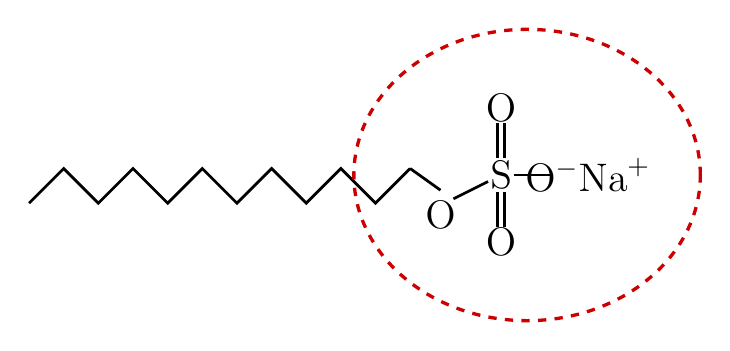
\begin{tikzpicture}[x=0.55cm, y=0.55cm, line width=1.0pt]
    % Chuỗi alkyl zigzag: CH3-(CH2)11-
    % 12 carbon: 0 to 11
    \draw (0,0) -- (0.8,0.8) -- (1.6,0) -- (2.4,0.8) -- (3.2,0) -- (4.0,0.8) -- (4.8,0) -- (5.6,0.8) -- (6.4,0) -- (7.2,0.8) -- (8.0,0) -- (8.8,0.8);
    % Nối tới O
    \draw (8.8,0.8) -- (9.5,0.3) node[below] {\Large O};
    
    % Từ O tới S
    \draw (9.8,0.1) -- (10.6,0.5);
    \node at (10.9,0.65) {\Large S};
    
    % Hai nhóm =O ở trên và dưới
    \draw[double, double distance=1.5pt] (10.9,1.05) -- (10.9,1.85);
    \node at (10.9,2.2) {\Large O};
    
    \draw[double, double distance=1.5pt] (10.9,0.25) -- (10.9,-0.55);
    \node at (10.9,-0.9) {\Large O};
    
    % Nhóm -O^- Na^+
    \draw (11.2,0.65) -- (12.1,0.65);
    \node at (12.9,0.65) {\Large O$^-\text{Na}^+$};
    
    % Vòng elip khoanh tròn nhóm ưa nước
    \draw[dashed, red!80!black, line width=1.2pt] (11.5,0.65) ellipse (2.2cm and 1.85cm);
\end{tikzpicture}
\end{document}
